%
% File acl2016.tex
%
%% Based on the style files for ACL-2015, with some improvements
%%  taken from the NAACL-2016 style
%% Based on the style files for ACL-2014, which were, in turn,
%% Based on the style files for ACL-2013, which were, in turn,
%% Based on the style files for ACL-2012, which were, in turn,
%% based on the style files for ACL-2011, which were, in turn,
%% based on the style files for ACL-2010, which were, in turn,
%% based on the style files for ACL-IJCNLP-2009, which were, in turn,
%% based on the style files for EACL-2009 and IJCNLP-2008...

%% Based on the style files for EACL 2006 by
%%e.agirre@ehu.es or Sergi.Balari@uab.es
%% and that of ACL 08 by Joakim Nivre and Noah Smith

\documentclass[11pt]{article}
\usepackage{acl2016}
\usepackage{times}
\usepackage{url}
\usepackage{latexsym}
\usepackage{breqn}

\usepackage{tikz}
\usetikzlibrary{bayesnet}

%\aclfinalcopy % Uncomment this line for the final submission
%\def\aclpaperid{***} %  Enter the acl Paper ID here

%\setlength\titlebox{5cm}
% You can expand the titlebox if you need extra space
% to show all the authors. Please do not make the titlebox
% smaller than 5cm (the original size); we will check this
% in the camera-ready version and ask you to change it back.

\newcommand\BibTeX{B{\sc ib}\TeX}

\title{Investigating the Sources of Linguistic Alignment in Conversation}
% \title{Investigating the Components of Linguistic Accommodation}

\author{First Author \\
  Affiliation / Address line 1 \\
  Affiliation / Address line 2 \\
  Affiliation / Address line 3 \\
  {\tt email@domain} \\\And
  Second Author \\
  Affiliation / Address line 1 \\
  Affiliation / Address line 2 \\
  Affiliation / Address line 3 \\
  {\tt email@domain} \\}

\date{}

\begin{document}
\maketitle

\begin{abstract}
In conversation, speakers tend to ``accommodate'' or ``align'' to their partners, changing the style and substance of their communications to be more similar to their partners' utterances. We focus here on ``linguistic alignment,'' changes in word choice based on others' choices. Although linguistic alignment is observed across many different contexts and its degree correlates with important social factors such as power and likability, its sources are still uncertain.
We build on a recent probabilistic model of alignment, using it to separate out alignment attributable to words versus word categories. We model alignment in two contexts: telephone conversations and microblog replies.
Our results show strong evidence of alignment, but it is primarily lexical rather than categorical. Furthermore, we find that discourse acts modulate alignment substantially. This evidence supports the view that alignment is shaped by strategic communicative processes related to the ongoing discourse.
\end{abstract}

\section{Introduction}

In conversation, people tend to adapt to one another across a broad range of behaviors. This adaptation behavior is collectively known as ``communication accommodation'' \cite{GilesCouplandCoupland1991}. Linguistic alignment, the use of similar words to a conversational partner, is one prominent form of accommodation. Alignment is found robustly across many settings, including in-person, computer-mediated, and web-based conversation \cite{DNMEtAl2012,GilesSchererTaylor1979,NiederhofferPennebaker2002}. In addition, the strength of alignment to conversational partners varies with important sociological factors, such as the power of the partners, their social network centrality, and their likability. Potentially, this alignment could be used to infer these factors in situations where they are difficult to observe directly.

Although linguistic alignment appears to reflect important social dynamics, the mechanisms underlying alignment are still not well-understood. One particular question is whether alignment is supported by relatively automatic priming mechanisms, or higher-level, discourse and communicative strategies. The Interactive Alignment Model proposes that conversational partners prime each other, causing alignment via the primed reuse of structures ranging from individual lexical items to syntactic abstractions  \cite{PickeringGarrod2004}. In contrast, Accommodation Theory emphasizes the relatively more communicative and strategic nature of alignment \cite{GilesCouplandCoupland1991}.

Relative to this theoretical landscape, a number of questions have emerged. First, does alignment occur at structural levels? If alignment is driven by interactive priming of structures, effects of alignment should be expected not only at the lexical level but also for structural elements or categories as well. In contrast, if alignment is primarily communicative, then alignment strength might differ and be greater for specific words that serve particular conversational or discourse functions in a particular situation.

Second, does alignment vary with conversational goals? If alignment is driven primarily by priming, it should be relatively consistent across different aspects of a discourse. In contrast, from a strategic or communicative perspective, alignment -- in which preceding words and concepts are reused -- must be balanced against a need to move the conversation forward by introducing new words and concepts. Thus, on a communicative account, alignment should be modulated by the speaker's discourse act, reflecting whether the balance of the concern is convergence on a current focus or conveyal of new information.

Our goal in the current work is to investigate these questions. We make use of a recent probabilistic model of linguistic alignment, modifying it to operate robustly over corpora with highly varying distributional structures and to consider both lexical and category-based alignment. We use two corpora of spontaneous conversations, the Switchboard Corpus and a corpus of Twitter conversations, to perform two experiments. First, in both datasets we measure alignment across different levels of representation and find very limited evidence for category-level alignment. Second, we make use of annotations in Switchboard to measure alignment across different discourse acts, finding that the level of alignment depends on the discourse actions that are included in the analysis. Taken together, these findings are consistent with the idea that alignment arises from discourse-level, strategic processes that operate primarily over lexical items.

\section{Previous Work}

\subsection{Why does alignment matter?}

Linguistic alignment, like other kinds of accommodation, can be a critical part of achieving social goals.  Performance in cooperative decision-making tasks is  positively related to the participants' linguistic convergence \cite{FusaroliEtAl2012,KacewiczEtAl2013}.  Romantically, match-making in speed dating and stability in established relationships have both been linked to increased alignment \cite{IrelandEtAl2011}. Alignment can also improve perceived persuasiveness, encouraging listeners to follow good health practices \cite{KlineCeropski1984} or to leave larger tips \cite{vanBaarenEtAl2003}.

Alignment is also important as an indicator of implicit sociological variables. Less powerful conversants generally accommodate to more to powerful conversants. Prominent examples include interviews and jury trials \cite{WillemynsEtAl1997,Gnisci2005,DNMEtAl2012}.  A similar effect is found for network structure: Speakers align more to more network-central speakers \cite{NobleFernandez2015}.  Additionally, factors such as gender, likability, respect, and attraction all interact with the magnitude of accommodation \cite{BilousKrauss1988,Natale1975}.
% Such differences in accommodation can also be indicative of changes to the power dynamic: In U.S. Supreme Court transcripts, \cite{guo2015} showed that depending on the accommodation dimension, justices -- who are more powerful by any intuitive assessment -- may nevertheless accommodate more to lawyers, perhaps because the lawyers have the local power to answer justices' questions.

\subsection{Sources of linguistic alignment}

Despite the important outcomes associated with alignment, its sources are not clear. The most prominent strand of work has focused on the level of word categories, looking at how interlocutors change their frequency of using, for instance, pronouns or quantitative words \cite{DNMEtAl2012,IrelandEtAl2011}. These results show alignment effects at the category level, but it is in principle possible that these effects arose purely from alignment on individual words (and that conclusion would not be inconsistent with the interpretation of that work).

Syntactic alignment is one area in which theoretical predictions have been tested, though results have been somewhat equivocal. The Interactive Alignment model has generally been taken to suggest that there should be cross-person priming of syntactic categories and structures \cite{PickeringGarrod2004}. But while some studies have found support for syntactic priming \cite{gries2005syntactic,dubey2005parallelism}, others have found negative or null alignment \cite{HealeyPurverHowes2014,reitter2010priming}. In one particularly thorough study, \cite{HealeyPurverHowes2014} find across two corpora that speakers syntactically \emph{diverged} from their interlocutors once lexical alignment was accounted for.

Furthermore, positive alignment is generally regarded as a good conversational tactic, but there is clearly a limit to its virtues, at least when it comes to content words. Alignment is inherently backward-looking, while the general goal of a conversation is to exchange information that is not already known by both parties, an inherently forward-looking goal. Perhaps because of this, some  recent work finding positive alignment has limited itself to ``non-topical'' word categories \cite{DNMGamonDumais2011,DoyleYurovskyFrank2016}. And suggestively, alignment within a task-relevant syntactic category was a better predictor of decision-making performance than overall lexical alignment \cite{FusaroliEtAl2012}.

In sum, although individual studies do bear on the sources of alignment, the picture is still not clear. Because most work on alignment has been done either on categories of words or aggregating across the lexicon, we do not have a good sense of whether there are systematic differences in alignment at different levels of representation. And a further important complication is that there is no one standard measure of alignment; we turn to this issue next.

\subsection{Measures of alignment}

The metrics used in previous work fall into two basic categories: distributional and conditional. Distributional methods such as Linguistic Style Matching (LSM) \cite{NiederhofferPennebaker2002,IrelandEtAl2011} or the Zelig Quotient \cite{JonesEtAl2014} calculate the similarity between the conversation participants over their frequencies of word or word category use in all utterances within the conversation. In contrast, conditional metrics, such as Local Linguistic Alignment (LLA) \cite{FusaroliEtAl2012,WangReitterYen2014} and the metric used by Danescu-Nicolescu-Mizil et al. \shortcite{DNMGamonDumais2011}, look at how a message conditions its reply, with alignment indicated by elevated word use in the reply when that word was in the preceding message.

While distributional methods have been popular, a major weakness of such methods is that they do not necessarily show true alignment, only similarity. A high level of distributional similarity does not imply that two conversational partners have aligned to one another, because they might instead have been similar to begin with. In contrast, conditional measures allow for stronger inferences about the temporal sequence of alignment (even though they cannot guarantee any causal interpretation). Thus, we focus here on conditional measures exclusively.
% The work reported here extends a recent conditional metric, the Hierarchical Alignment Model, or HAM \cite{DoyleYurovskyFrank2016}.

%\paragraph{Distributional methods} [LSM overview]

\paragraph{By-message conditional methods} Several existing conditional methods have started from the simplified representation that messages either do or do not contain particular words ("markers"), irrespective of message length or marker count. \cite{DNMEtAl2012,DoyleYurovskyFrank2016}. We refer to these as ``by message" methods. Consider the following example of conditional alignment, using pronouns as the marker: Bob aligns to Alice if his replies are more likely to contain a pronoun when in response to a message from Alice that contains a pronoun.

\begin{center}
\begin{tabular}{|c||c|c|}
\hline
& \multicolumn{2}{|c|}{Bob's reply} \\
\hline
Alice's message & has pronoun & no pronoun \\ \hline
has pronoun & 8 & 2\\
no pronoun & 5 & 5\\
\hline
\end{tabular}
\end{center}

Here, Alice sends 10 messages that contain at least one pronoun, and 8 of Bob's replies contain at least one pronoun.  But Alice also sends 10 messages that don't contain any pronouns, and only 5 of Bob's replies to these contain pronouns. This increased likelihood of a pronoun-containing reply to a pronoun-containing message is the conditional alignment.

Different models quantify this conditional alignment slightly differently.  Danescu-Niculescu-Mizil et al.~\shortcite{DNMGamonDumais2011} proposed a subtractive conditional probability model, where alignment is the difference between the likelihood of a pronoun-containing reply $B$ to a pronoun-containing message $A$ and the probability of a pronoun-containing reply to any message:\vspace*{-5pt}

\begin{equation}
align_{SCP} = p(B|A) - p(B)
\end{equation}

Doyle, Yurovsky, and Frank \shortcite{DoyleYurovskyFrank2016} showed that this measure can be affected by the overall frequency of the category being aligned on, though. To correct this issue, they proposed a Hierarchical Alignment Model (HAM), which defines alignment as a linear effect on the log-odds of a reply containing the relevant marker (e.g., a pronoun), similar to a linear predictor in a logistic regression.\footnote{Because the HAM estimated this quantity via Bayesian inference, the inferred alignment value depends on the prior and number of messages observed, so unlike the other measures, this equality is only approximate.}\vspace*{-5pt}

\begin{dmath}
align_{HAM} \approx logit^{-1}(p(B|A)) - \\ \hspace*{1.2em} logit^{-1}(p(B|\neg A))
\end{dmath}

These binary conditional methods depend on the assumption that all messages have similar, and small, numbers of words, however. The probability that a message contains at least one of any marker of interest is dependent on the message's length, so if messages vary substantially in their length, these alignment values can be at least noisy, if not biased. They are also not robust as messages increase in length, since the likelihood that a message contains any marker approaches 1 as message length increases.

\paragraph{By-word conditional methods} A solution to the problem of variable message lengths is simply to shift from binarized data to count data. Instead of counting how many times Bob's replies contain at least one pronoun, we can count what proportion of his replies' word tokens are pronouns.  Some existing measures use a related quantity, the proportion of the preceding message that appears in its reply, to estimate alignment, notably Local Linguistic Alignment (LLA) \cite{FusaroliEtAl2012,WangReitterYen2014} and the lexical similarity (LS) measure of \cite{HealeyPurverHowes2014}. LLA is defined as the number of word tokens ($w_i$) that appear in both the message ($M_a$) and the reply ($M_b$), divided by the product of the total number of word tokens in the message and reply:\vspace*{-5pt}

\begin{equation}
align_{LLA} = \frac{\sum_{w_i \in M_b} \delta(w_i \in M_a)}{length(M_a)length(M_b)}
\end{equation}

These measures have an aspect of conditionality, as they only count words that appear in both the message and the reply. But they nevertheless fail to control for the baseline frequency of the initial marker, and hence may be biased in measurements across words or categories of different frequencies \cite{DoyleYurovskyFrank2016}. They also can be affected by reply length, as the maximum alignment estimate is only possible when the reply is shorter than the message.
% \footnote{Proof in Supplemental?}
% AM outperformed SCP, LLA, and LSM in simulations in \cite{DoyleYurovskyFrank2016}
An better measure would have the benefits of the existing by-message conditional models and the length-robustness of a by-word conditional method. We present a modification of the HAM model satisfies this goal.

\section{The Word-Based Hierarchical Alignment Model (WHAM)}

% The HAM framework conceptualizes alignment as the increase in the likelihood that a reply will contain a ``marker''---a word or word category---given that the preceding message contained it, compared to when the preceding message did not contain it. This introduces a substantial simplification: it treats each message as a binary variable, either containing or not containing the word of interest. By-message alignment has successfully found alignment effects in previous work \cite{DNMGamonDumais2011}, and may be appropriate for data such as the Twitter dataset used in that paper. However, in looking at more natural dialogues, such as telephone conversations, length may vary substantially between messages, obscuring the alignment effect.

We propose the Word-Based Hierarchical Alignment Model (WHAM). Like HAM, WHAM  assumes that word use in replies is shaped by whether the preceding message contained the marker of interest. But WHAM models marker token frequencies within replies, so that a 40-word reply with two instances of the marker is represented differently from a 3-word reply containing with one instance.

For each marker, WHAM treats each reply as a series of token-by-token independent draws from a binomial distribution. The binomial probability is dependent on whether the preceding message did ($\mu^{align}$) or did not ($\mu^{base}$) contain the marker, and the inferred alignment value is the difference between these probabilities in log-odds space ($\eta^{align}$). The graphical model is shown in Figure \ref{fig:wham}.

\begin{figure*}[t]
  \begin{center}
    % model_lda.tex
%
% Copyright (C) 2010,2011 Laura Dietz
% Copyright (C) 2012 Jaakko Luttinen
%
% This file may be distributed and/or modified
%
% 1. under the LaTeX Project Public License and/or
% 2. under the GNU General Public License.
%
% See the files LICENSE_LPPL and LICENSE_GPL for more details.

% Latent Diriclet allocation model

%\beginpgfgraphicnamed{model-lda}
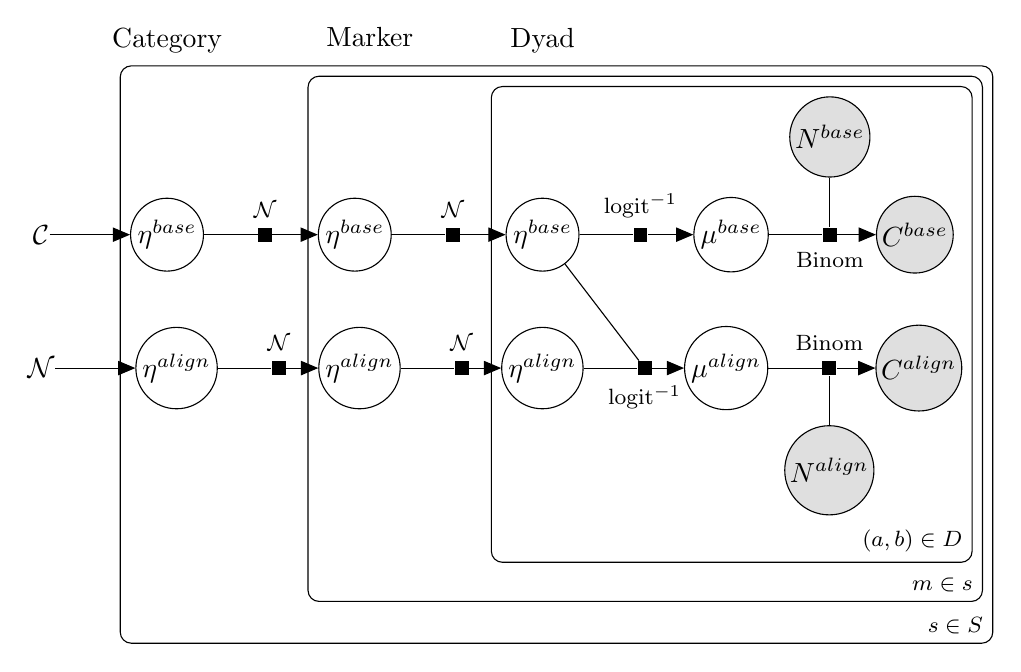
\begin{tikzpicture}[x=1.7cm,y=1.8cm]

  % Nodes

  \node[const] (base) {$\mathcal{C}$};
%  \node[latent,right=.6 of base] (n_b_m) {$\eta^{base}_m$};
%  \node[latent,right=.8 of n_b_m] (n_b_ms) {$\eta^{base}_{m,s}$};
%  \node[latent,right=.8 of n_b_ms] (n_b_mab) {$\eta^{base}_{m,a,b}$};
%  \node[latent,right=.8 of n_b_mab] (m_b_mab) {$\mu^{base}_{m,a,b}$};
%  \node[obs,right=.8 of m_b_mab] (C_b_mab) {$C^{base}_{m,a,b}$};

  \node[const,below=.8 of base] (align) {$\mathcal{N}$};
% \node[latent,right=.6 of align] (n_a_m) {$\eta^{align}_m$};
% \node[latent,right=.75 of n_a_m] (n_a_ms) {$\eta^{align}_{m,s}$};
% \node[latent,right=.75 of n_a_ms] (n_a_mab) {$\eta^{align}_{m,a,b}$};
% \node[latent,right=.75 of n_a_mab] (m_a_mab) {$\mu^{align}_{m,a,b}$};
% \node[obs,right=.8 of m_a_mab] (C_a_mab) {$C^{align}_{m,a,b}$};

  \node[latent,right=.6 of base] (n_b_m) {$\eta^{base}$};
  \node[latent,right=.85 of n_b_m] (n_b_ms) {$\eta^{base}$};
  \node[latent,right=.85 of n_b_ms] (n_b_mab) {$\eta^{base}$};
  \node[latent,right=.85 of n_b_mab] (m_b_mab) {$\mu^{base}$};
  \node[obs,right=.8 of m_b_mab] (C_b_mab) {$C^{base}$};

  \node[latent,right=.6 of align] (n_a_m) {$\eta^{align}$};
  \node[latent,right=.75 of n_a_m] (n_a_ms) {$\eta^{align}$};
  \node[latent,right=.75 of n_a_ms] (n_a_mab) {$\eta^{align}$};
  \node[latent,right=.75 of n_a_mab] (m_a_mab) {$\mu^{align}$};
  \node[obs,right=.8 of m_a_mab] (C_a_mab) {$C^{align}$};


  \node[const,above=1.02 of n_b_m] (marker) {Category};
  \node[const,above=1.06 of n_b_ms] (group) {\hspace{.75em} Marker};
  \node[const,above=1.02 of n_b_mab] (dyad) {Dyad};

  % Factors

  \factor[right=of n_b_m] {n_b_m_f} {above:$\mathcal{N}$} {} {};
  \factor[right=of n_b_ms] {n_b_ms_f} {above:$\mathcal{N}$} {} {};
  \factor[right=of n_b_mab] {n_b_mab_f} {above:$\textrm{logit}^{-1}$} {} {};
  \factor[right=of m_b_mab] {m_b_mab_f} {below:Binom} {} {};

  \factor[right=of n_a_m] {n_a_m_f} {above:$\mathcal{N}$} {} {};
  \factor[right=of n_a_ms] {n_a_ms_f} {above:$\mathcal{N}$} {} {};
  \factor[right=of n_a_mab] {n_a_mab_f} {below:$\textrm{logit}^{-1}$} {} {};
  \factor[right=of m_a_mab] {m_a_mab_f} {above:Binom} {} {};

  %\factor[right=of C_b_mab] {C_b_mab_f} {above:Binom$} {} {};

  %\factor[above=of X]     {X-f}     {Multi} {} {} ; %
  %\factor[above=of T]     {T-f}     {left:Multi} {} {} ; %
  %\factor[above=of theta] {theta-f} {left:Dir} {} {} ; %

  % More nodes
  %\node[latent, right=of X-f] (phi)  {$\phi$}; %
  %\node[const, above=of phi]  (aphi) {$\alpha_\phi$}; %

  %\factor[above=of phi] {phi-f} {right:Dir} {} {} ; %

%  \node[obs,above=.35 of m_b_mab_f] (N_b_mab) {$N^{base}_{m,a,b}$};
%  \node[obs,below=.35 of m_a_mab_f] (N_a_mab) {$N^{align}_{m,a,b}$};

  \node[obs,above=.35 of m_b_mab_f] (N_b_mab) {$N^{base}$};
  \node[obs,below=.35 of m_a_mab_f] (N_a_mab) {$N^{align}$};


  \edge{base}{n_b_m};
  \factoredge {n_b_m}  {n_b_m_f}     {n_b_ms} ; %
  \factoredge {n_b_ms}  {n_b_ms_f}     {n_b_mab} ; %
  \factoredge {n_b_mab}  {n_b_mab_f}     {m_b_mab} ; %
  \factoredge {m_b_mab,N_b_mab} {m_b_mab_f} {C_b_mab}; %

   \edge{align}{n_a_m};
  \factoredge {n_a_m}  {n_a_m_f}     {n_a_ms} ; %
  \factoredge {n_a_ms}  {n_a_ms_f}     {n_a_mab} ; %
  \factoredge {n_a_mab,n_b_mab}  {n_a_mab_f}     {m_a_mab} ; %
  \factoredge {m_a_mab,N_a_mab} {m_a_mab_f} {C_a_mab}; %
 %\factoredge {atheta} {theta-f} {theta} ; %
  %\factoredge {phi}    {X-f}     {X} ; %
  %\factoredge {aphi}   {phi-f}   {phi} ; %

  %\gate {X-gate} {(X-f)(X-f-caption)} {T}

  \plate {pairplate} { %
    (N_b_mab)(C_b_mab) %
    (m_b_mab)(n_b_mab) %
    (N_a_mab)(C_a_mab) %
    (m_a_mab)(n_a_mab) %
  } {$(a,b) \in D$}; %
  \plate {subpopplate} { %
    (pairplate) %
    (n_b_ms) (n_a_ms) %
  } {$m \in s$} ; %
  \plate {} { %
    (subpopplate) %
    (n_b_m) (n_a_m)
  } {$s \in S$} ; %

\end{tikzpicture}
%\endpgfgraphicnamed

%%% Local Variables:
%%% mode: tex-pdf
%%% TeX-master: "example"
%%% End:

  \end{center}
  \caption{The Word-Based Hierarchical Alignment Model (WHAM). A chain of normal distributions generates a linear predictor $\eta$, which is converted into a probability $\mu$ for binomial draws of the words in each reply.}\label{fig:wham}
\end{figure*}

For a set of message-reply pairs between a speaker-replier dyad $(a,b)$, we first separate the replies into two sets based on whether the preceding message contained the marker $m$ (the ``alignment'' set) or not (the ``baseline'' set). All replies within a set are then aggregated in a single bag-of-words representation, with marker token counts $C^{align}_{m,a,b}$ and $C^{base}_{m,a,b}$, and total token counts $N^{base}_{m,a,b}$ and $N^{base}_{m,a,b}$, the observed variables on the far right of the model.  Moving from right to left, these counts are assumed to come from binomial draws with probability $\mu^{align}_{m,a,b}$ or $\mu^{base}_{m,a,b}$.  The $\mu$ values are generated from $\eta$ values in log-odds space by an inverse-logit transform, similar to linear predictors in logistic regression.

The $\eta^{base}$ variables are representations of the baseline frequency of a marker in log-odds space, and $\mu^{base}$ is simply a conversion of $\eta^{base}$ to probability space, the equivalent of an intercept term in a logistic regression. $\eta^{align}$ is an additive value, with $\mu^{align} = \textrm{logit}^{-1}(\eta^{base}+\eta^{align})$, the equivalent of a binary feature coefficient in a logistic regression.  Alignment is then the change in log-odds of the replier using $m$ above baseline usage, given that the initial message uses $m$.

The remainder of the model is a hierarchy of normal distributions that allow social and word category structure to be integrated into the analysis. In the present work, we have three levels in the hierarchy: category level, marker level,\footnote{In the lexical and category-not-word alignment models, these markers are words within a category. The category alignment model does not include this level, since all words in a category are treated identically.} and conversational dyad level. All of these normal distributions have identical standard deviations $\sigma^2=.25$.\footnote{This value was chosen as a good balance between reasonable parameter convergence (improved by smaller $\sigma^2$) and good model log-probability (improved by larger $\sigma^2$).}  A $Cauchy(0,2.5)$ distribution gives a relatively uninformative prior for baseline marker frequency \cite{GelmanEtAl2008}. The alignment hierarchy is headed by a normal distribution centered at 0, biasing the model equally in favor of positive and negative alignments.

% The key quantity for our analyses is the category-level variable $\eta^{align}_{S}$, the level of alignment on category $S$ across all dyads.

%\begin{center}
%\begin{tabular}{|c|}
%\hline
%Generative Model \\
%\hline
%Alice says $x$, Bob wants to reply. \\
%If $m \not\in x$, then $p(B_m|A_m) = \mu^{base}(m)$ \\
%If $m \in x$, then $p(B_m|\neg A_m) = \mu^{align}(m)$ \\
%\hline
%$\mu^{base}(m) = logit^{-1}(\eta^{base}(m))$ \\
%$\mu^{align}(m) = logit^{-1}(\eta^{base}(m)+\eta^{align}(m))$ \\
%\hline
%\end{tabular}
%\end{center}

For our marker set, we adopt the Linguistic Inquiry and Word Count (LIWC) system to categorize words \cite{LIWC}.  We use a set of 11 categories that have shown alignment effects in previous work \cite{DNMGamonDumais2011}. These can be loosely grouped into a set of five syntactic categories (articles, conjunctions, prepositions, pronouns, and quantifiers) and six conceptual categories (certainty, discrepancy, exclusion, inclusion, negation, and tentative). Categories and example elements are shown in Table \ref{table:liwc}. We manually lemmatized all words in each category.

We implemented WHAM in RStan \cite{Stan}, with code available at \url{http://github.com/langcog/disc_align}.

\begin{table}
\centering
\small
\begin{tabular}{|c|c|c|c|c|} \hline
& & & Swbd & Twit \\
Category & Examples & Size & Prob & Prob\\ \hline
Article & \textit{a, the} & 2 & .053 & .047\\
Certainty  & \textit{always, never} & 17 & .014 & .015\\
Conjunction  & \textit{but, and, though} & 18 & .077 & .051\\
Discrepancy  & \textit{should, would} & 21 & .015 & .019\\
Exclusive  & \textit{without, exclude} & 77 & .038 & .028\\
Inclusive  & \textit{with, include} & 57 & .057 & .028\\
Negation  & \textit{not, never} & 12 & .020 & .023\\
Preposition  & \textit{to, in, by, from} & 97 & .097 & .091\\
Pronoun   & \textit{it, you} & 55 & .17 & .16\\
Quantifier  & \textit{few, many} & 23 & .028 & .025\\
Tentative & \textit{maybe, perhaps} & 28 & .033 & .025\\
\hline\end{tabular}
\caption{Marker categories for linguistic alignment, with examples, number of distinct word lemmas, and token probability of in a reply in Switchboard and Twitter.}\label{table:liwc}
\end{table}

\section{Data}

We use two corpora for our experiments. The first is a collection of Twitter conversations collected by Doyle \& Frank \shortcite{DoyleFrank2015CMCL} to examine information density in conversation. This corpus focuses on conversations within a set of 14 mostly distinct sub-communities on Twitter, and contains 63,673 conversation threads, covering 228,923 total tweets.  We divide these conversations into message pairs, also called conversational turns, which are two consecutive tweets within a conversation thread.  The second tweet is always in reply to the first (according to the Twitter API), although this does not necessarily mean that the content of the reply is a response to the preceding tweet. Retweets (including explicit retweets and some common manual retweet methods) were removed automatically. This processing leaves us with 122,693 message pairs, spanning 2,815 users.  The tweets were parsed into word tokens using the Twokenizer \cite{OwoputiEtAl2013}.

The second corpus is the SwDA version of the Switchboard corpus \cite{godfrey1992switchboard,jurafsky1997switchboard}.\footnote{Available courtesy of Christopher Potts at \url{http://compprag.christopherpotts.net/swda.html}.} This corpus is a collection of transcribed telephone conversations, with each utterance labeled with the discourse act it is performing (e.g., statement of opinion, signal of non-understanding).  It contains 221,616 total utterances in 1,155 conversations.  We combine consecutive utterances by the same speaker without interruption from the listener into a single message and treat consecutive pairs of messages from different speakers as conversation turns, resulting in 110,615 message pairs.

\section{Experiment 1: Lexical- and Category-Level Alignment}
%
% We perform two experiments. First, we look at how lexical-level and category-level alignment interact, and find that on Twitter and telephone conversations, lexical alignment dominates categorical alignment.  We then use the telephone conversations to investigate the effect of discourse structure on alignment, focusing on the effect of backchannels.

% \subsection{Experiment 1}

Our first experiment examines how alignment differs across the lexical and categorical levels. We use the WHAM framework to infer alignment on word and category counts, and also introduce a measure to estimate the influence of one word in a category on other words in its category, ``category-not-word'' alignment. We include this last type of alignment because it is possible that the category alignment effects in previous work are the result of lexical alignment on the individual words in the category, without any influence across words in the category. If categorical alignment is a real effect over and above lexical alignment, then the presence of a word in a message should not only increase the chance of seeing that word in the reply, but also other words in its category.


% Furthermore, we are interested in explicitly tracking the influence of lexical alignment on categorical alignment.

% \subsubsection{Levels of alignment and their interaction}

% We want to examine the interaction of two levels of alignment. The first is lexical-level alignment, looking at how the presence of a word (lemma) in a message increases its likelihood of appearing in the reply.  The second is category-level alignment, looking at how the presence of a member of a word category in a message increases the likelihood of words from that category appearing in the reply.  These categories generally correspond to syntactic classes (pronouns, conjunctions) or broad conceptual classes (inclusive words, negative emotions)   Work on by-word conditional alignment has tended to focus on the lexical level, while distributional and by-message conditional alignment work has focused on the categorical level.

%Some recent work has explored interactions between these levels. \cite{HealeyPurverHowes2014} treat lexical alignment as the baseline and find that turn-by-turn syntactic alignment is actually slightly lower than lexical alignment would predict. On the other hand, \cite{XuReitter2015} argue for LLA as a good alignment measure in part because of its high correlation between lexical and syntactic alignment, under the assumption that alignment at all levels is a communicative goal \cite{PickeringGarrod2004}. A major goal of this experiment is thus to investigate whether lexical- and categorical-level alignment point in the same direction.


%Intuitively, category alignment must be no less than the mean lexical alignment of words in the category, since each instance of lexical agreement is also an instance of category agreement.\footnote{More precisely, the weighted mean given lexical frequency.}

\subsection{Category-not-word-alignment model}

\begin{table}[t]
\begin{center}
\begin{tabular}{|c||c|c|c|}
\hline
& \multicolumn{3}{|c|}{\bf Reply} \\
\hline
\bf Message & $\emptyset$ & \textit{he} & \textit{she} \\ \hline
$\emptyset$ & 25 & 25 & 25\\
\textit{he} & 20 & 50 & 10 \\
\textit{she} & 20 & 10 & 50 \\
\hline
\end{tabular}
\end{center}
\caption{\label{table:cnw-example1} A theoretical case where lexical alignment surpasses categorical alignment due to negative CNW between the words.}
\end{table}

Assessing the amount of alignment triggered across words in a category (which we call ``category-not-word alignment'' or CNW) is not trivial, as there are a variety of interactions between lexical items within a category that can cause the lexical alignment to actually be less than the category alignment. Table \ref{table:cnw-example1} illustrates this with a theoretical distribution over the pronouns \textit{he} and \textit{she}; one use of the pronoun \textit{he} makes another use more likely (\textit{Did he like the movie? Yeah, he loved it.}) while also reducing the likelihood of \textit{she}, since the topic of conversation is now a male, and vice versa for \textit{she}. For both \textit{he} and \textit{she}, the lexical alignment is approximately $logit^{-1}(p(B|A)-p(B|\neg A)) = logit^{-1}(\frac{50}{80}-\frac{25}{75}) \approx 1.2$,
but categorical alignment is approximately $logit^{-1}(\frac{120}{160}-\frac{50}{75}) \approx 0.4$. On the other hand, the pronouns \textit{you} and \textit{I} might trigger each other more than themselves (\textit{A: Did you like the movie? B: Yeah, I loved it.}).


% Lexical alignment can differ from categorical alignment for a variety of reasons, so we consider three quantities: the lexical and categorical alignments, but also the ``category-not-word'' (CNW) alignment: the increased likelihood of seeing another member of the category other than the target word.

% \subsection{Category-not-word Alignment}


% \begin{table}[t]
% \begin{center}
% \begin{tabular}{|c||c|c|c|}
% \hline
% & \multicolumn{3}{|c|}{\bf Reply} \\
% \hline
% \bf Message & $\emptyset$ & \textit{you} & \textit{I} \\ \hline
% $\emptyset$ & 25 & 25 & 25\\
% \textit{you} & 20 & 10 & 50 \\
% \textit{I} & 20 & 50 & 10 \\
% \hline
% \end{tabular}
% \end{center}
% \caption{A theoretical case where lexical alignment is below categorical alignment due to greater CNW alignment between the words than lexical alignment.}
% \end{table}

To investigate CNW alignment, we look at a subset of the data: for each word $w$, exclude all messages that contain a word from that category ($S$) that is not $w$. This limits the category alignment influence on the reply to the single word $w$. Then, instead of looking at how often $w$ appears in the reply, we look at how often \emph{all other words} in category $S$ appear in the reply.  The model then infers the influence of $w$ on the other words in the category independent of their lexical alignment. Within the WHAM model, we change the count variables $C^\cdot$ and $N^\cdot$ so that $C^{align}$ is the number of tokens of $\{S-w\}$ in replies to messages containing $w$ but not $\{S - w\}$. $C^{base}$ is then the number in replies to messages not containing any words in $S$.  Similarly, $N^{align}$ is the total token counts over replies containing $w$ but not any other words in $S$, and $N^{base}$ the total token counts over replies containing no words in $S$.

\subsection{Methods}

We conducted three sets of simulations, fitting the model with marker categories, individual words, and with the CNW scheme described above.
In each, the model was fit with two chains of 200 iterations of the sampler for each dataset.  We then extracted alignment estimates from each of the final 100 samples, and we report 95\% highest posterior density intervals on  $\eta^{align}_S$. %in Figures \ref{fig:twitter-res} and \ref{fig:swbda-res}.

\subsection{Results}


\begin{figure*}[t]
  \begin{center}
    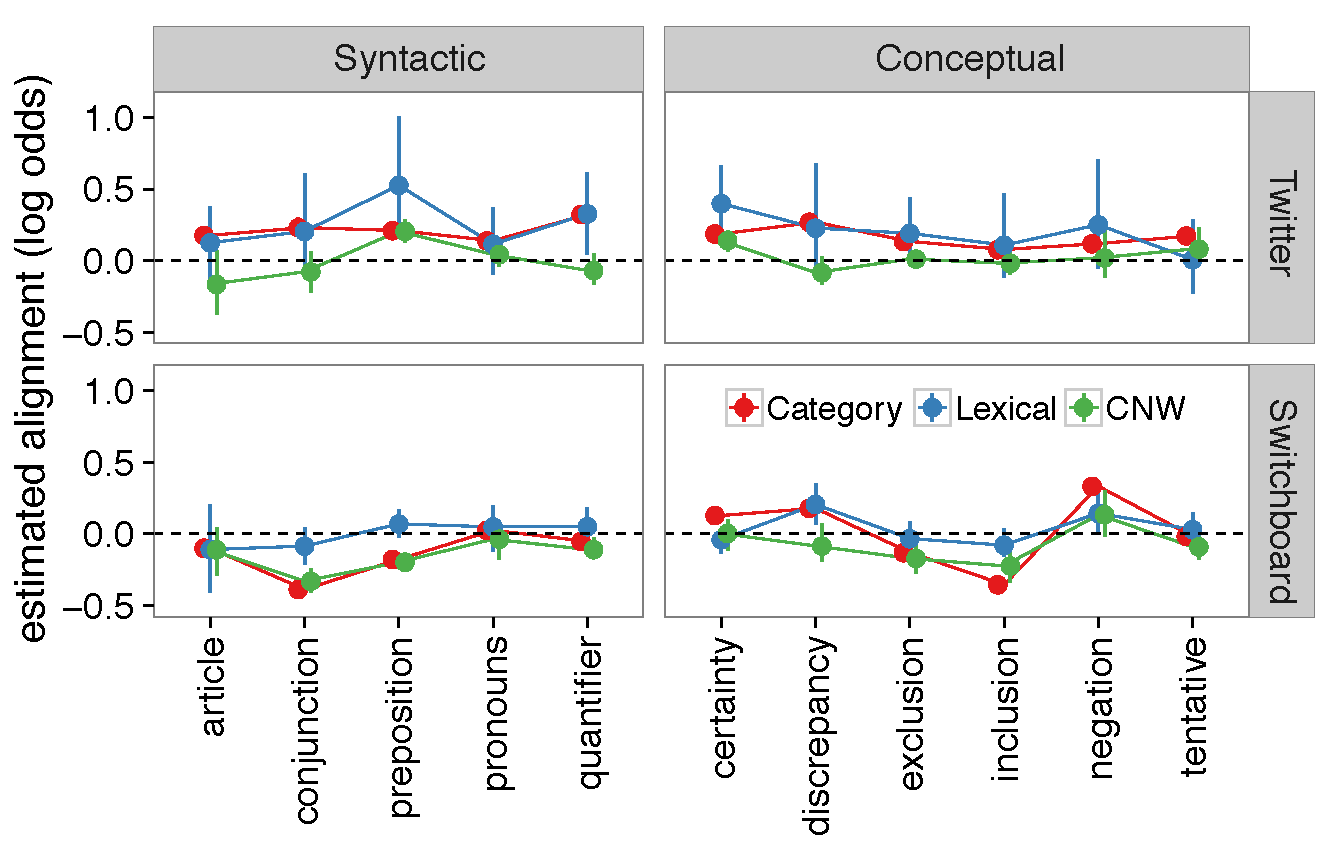
\includegraphics[width=1.5\columnwidth]{results/twitter_swbda_mod.pdf}
  \end{center}
  \caption{(left) Categorical (red), lexical (blue), and CNW (green) alignments plotted by category, on the Twitter (left) and Switchboard (right) datasets. 95\% HPD intervals from WHAM shown.}\label{fig:all-res}
\end{figure*}

%
% \begin{figure}[t]
%   \begin{center}
%     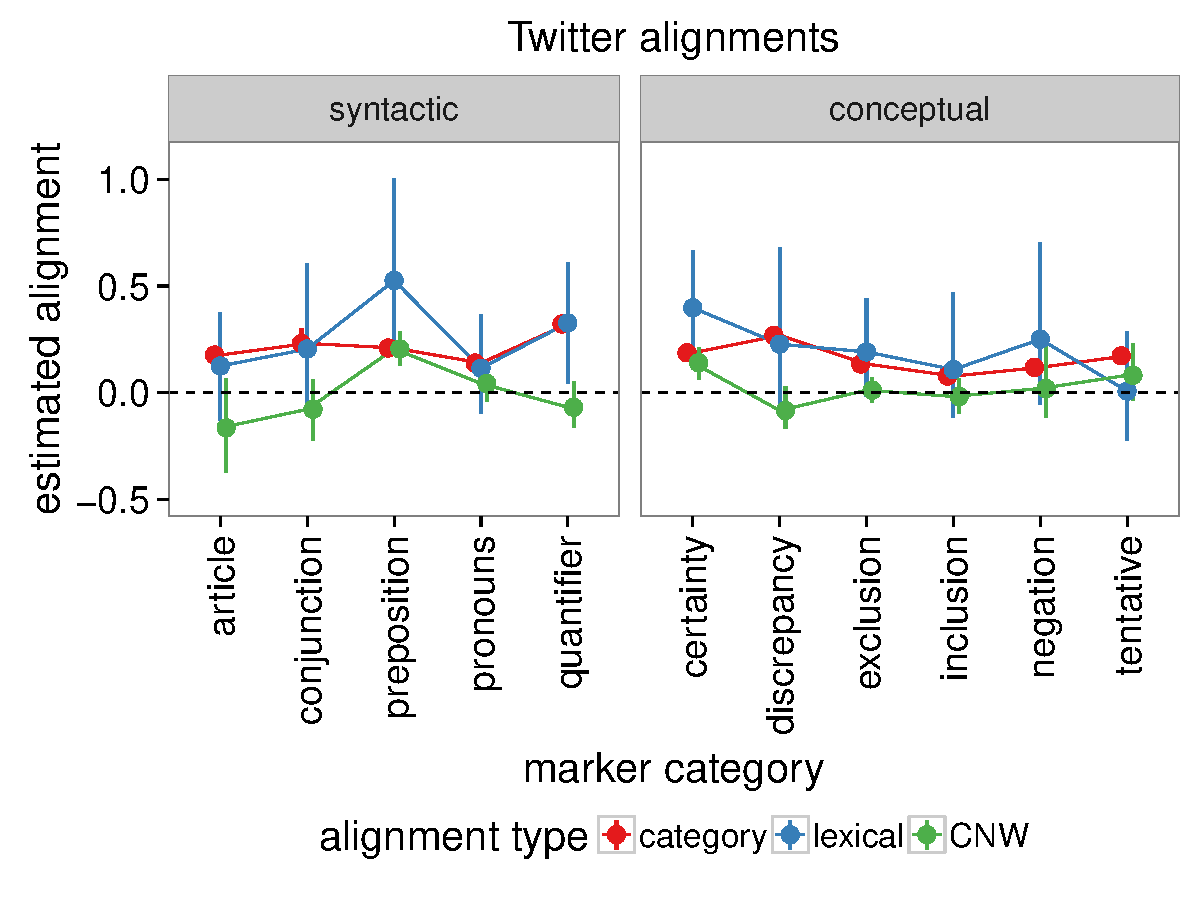
\includegraphics[width=\columnwidth]{results/twitter_line.pdf}
%   \end{center}
%   \caption{Categorical (red), lexical (blue), and CNW (green) alignments on the Twitter dataset. 95\% HPD intervals from WHAM shown.}\label{fig:twitter-res}
% \end{figure}
%
% \begin{figure}[t]
%   \begin{center}
%     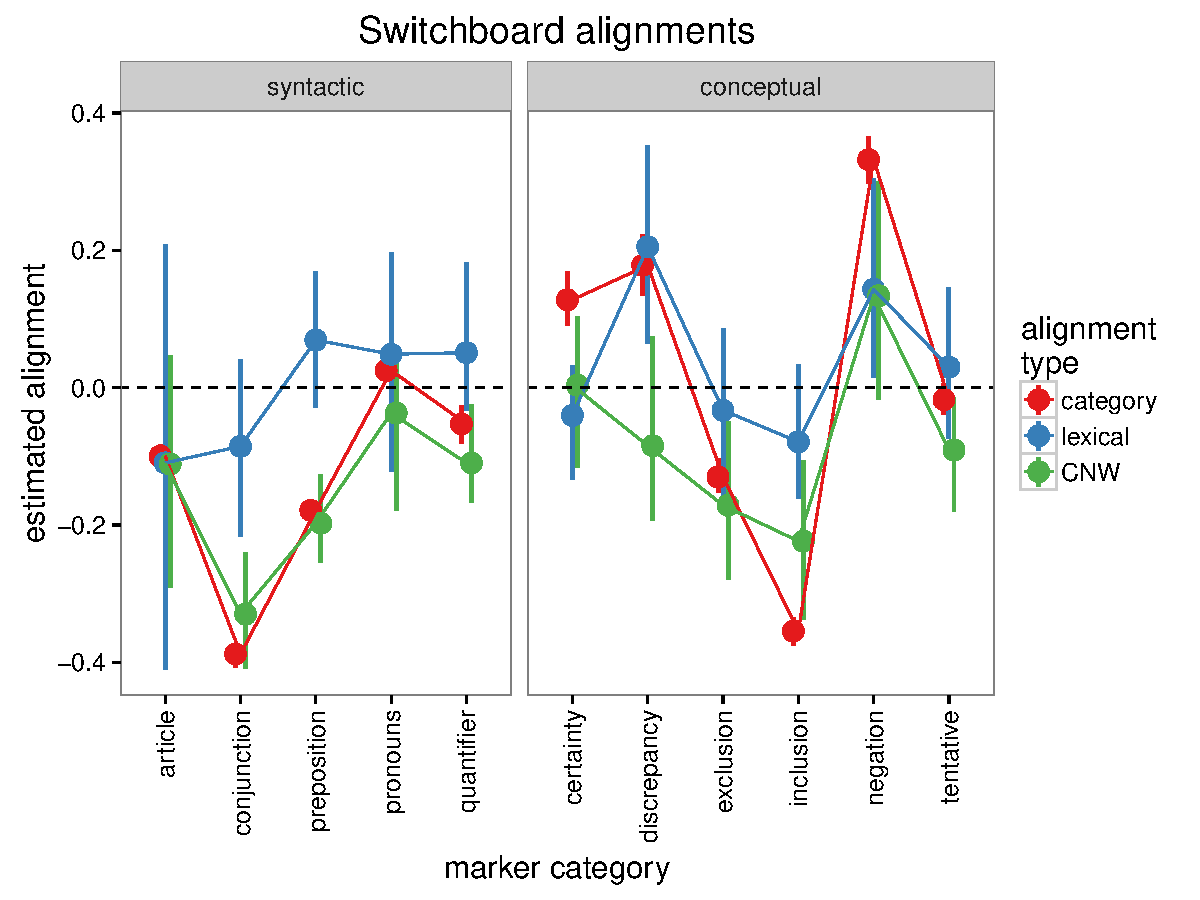
\includegraphics[width=\columnwidth]{results/swbda_line.pdf}
%   \end{center}
%   \caption{Categorical (red), lexical (blue), and CNW (green) alignments on the Switchboard dataset. 95\% HPD intervals from WHAM shown.}\label{fig:swbda-res}
% \end{figure}

Figure \ref{fig:all-res} shows the alignment on each marker category in the Twitter and Switchboard corpora. There were substantial differences in the overall rate of alignment between the corpora: Mean category alignment on Twitter was $.19$, while Switchboard category alignment was $-.051$. These differences may reflect the nature of the two discourse contexts: Replies on Twitter are composed while looking at the preceding message, encouraging the replier to take more account of the other tweeter's words, and a replier can draft and edit their reply to make it better fit the conversation.  Messages on Switchboard, on the other hand, are evanescent, so a replier must compose a reply without looking back at the message, without editing, and in real-time. Differences in the discourse structure of these corpora may also be contributing, an effect we will consider in Experiment 2.  %In Experiment 2, we will show that differences in discourse structure may also impact the differences in alignment.

Despite the difference in reply construction in the two corpora, the results across levels of alignment were similar. Alignment was found primarily at the lexical -- rather than the category -- level. Lexical and category alignment were not significantly different from each other, but the strength of lexical alignment was significantly larger than the CNW alignment, according to a $t$-test over categories (Twitter: $t(10)=.21, p<.001$; Swbd: $t(10)=.12,p=.003$). CNW alignment was significantly negative on Switchboard ($t(10)=-.11, p=.01$) and not significantly different from zero on Twitter ($t(10)=.009, p=.79$).

WHAM -- unlike other previous measures -- provides estimates of alignment that are unbiased by either marker frequency or message length, but we still observed modest alignment on Twitter, replicating previous work \cite{DoyleYurovskyFrank2016,DNMGamonDumais2011}. Alignment was smaller in Switchboard, and in both cases there were no category effects. Thus, the categorical alignment results may result primarily from lexical alignment, inconsistent with the predictions of interactive priming accounts of alignment.

%The two corpora also differ in the correlations between the alignment measures. The Switchboard corpus, despite its overall tendency against category alignment, has significant positive correlations between category and lexical ($r = .71, p=.015$), and category and CNW alignment ($r = .94, p <.001$), as well as marginal positive alignment between lexical and CNW alignment ($r = .52, p = .10$).  This suggests a consistency across words within a category on Switchboard


\section{Experiment 2: Discourse Acts and Alignment}

% \subsubsection{Discourse Acts}
Messages within a discourse can serve a very wide range of purposes. This variety has effects for both linguistic structure and the relationship to neighboring messages. For example, a simple yes/no question is likely to receive a short, constrained reply, while a statement of an opinion is more likely to yield a longer reply. In addition, different types of messages can either introduce new information to the conversation (e.g., statements, questions, offers) or look back at existing information (e.g., acknowledgments, reformulations, yes/no answers). We hypothesize that alignment will be substantially different depending on the discourse act, as speakers' conversational goals vary. Thus, our second experiment examines how alignment differs depending on discourse act.
% In particular, we are interested in how alignment is modulated by the discourse goal and the flexibility in the form of an utterance.

We focus on a particular kind of discourse act, the backchannel \cite{Yngve1970}. Backchannels are extremely common in Switchboard, accounting for almost 20\% of utterances, and include utterances such as single words signaling understanding or misunderstanding (\textit{yeah, uh-huh, no}) or simple messages expressing empathy without trying to take a full conversational turn (\textit{It must have been tough}).  Backchannels are a particularly interesting case because their short and constrained nature makes it difficult to align on some categories (e.g., backchannels rarely contain quantifiers or prepositions), while the purpose of giving feedback to the speaker makes it important to align on others (e.g., matching the positive/negative tone or certainty of a speaker).  In addition, backchannels are primarily restricted to spoken corpora. Twitter conversations contain far fewer backchannels than Switchboard, which may account for some of their alignment differences---especially as the results of this experiment suggest that backchannels reduce overall alignment.

% We expect that alignment will increase for most categories, although categories that are important in backchannels may decrease.


\subsection{Methods}

We use the discourse-annotated Switchboard corpus to compare alignment in conversations containing backchannels with those whose backchannels have been removed. We make this comparison by creating a second corpus, removing every utterance classified as a backchannel from the corpus prior to parsing the utterances into conversation turns as before.
% Twitter data is not used as we do not have discourse act annotations on it.

\begin{figure}[t]
  \begin{center}
    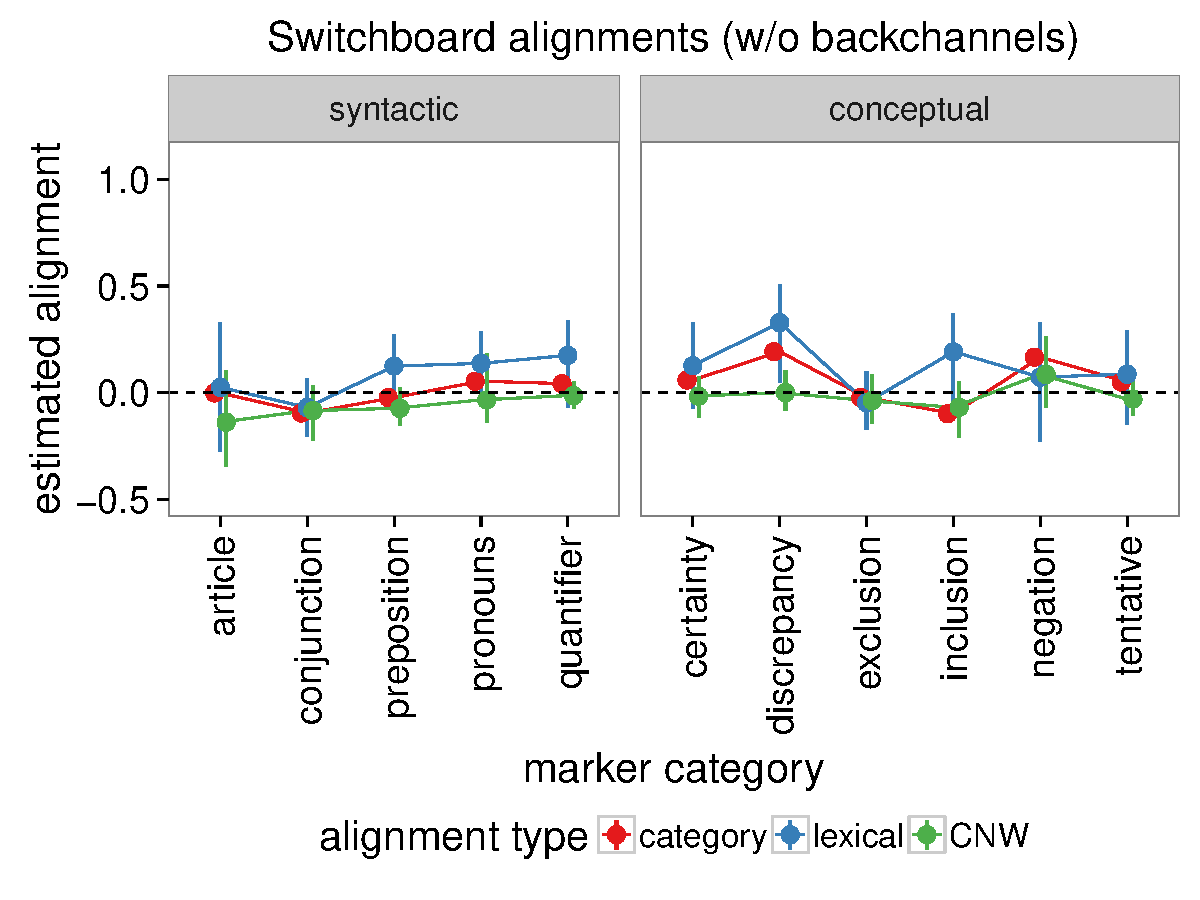
\includegraphics[width=\columnwidth]{results/swbdn_line.pdf}\vspace{-10pt}
  \end{center}
  \caption{Categorical (red), lexical (blue), and CNW (green) alignments on the Switchboard dataset with backchannels removed. 95\% HPD intervals from WHAM shown.}\label{fig:swbdn-res}
\end{figure}


\subsection{Results}

Alignment values for the Switchboard corpus without backchannels are shown in Figure \ref{fig:swbdn-res}. As expected, alignment is on average higher without the backchannels ($p=.09$ for category, $p<.05$ for lexical and CNW), reflecting the constrained nature of backchannels. Lexical alignment is significantly higher than category alignment ($t(10) =-.08, p = .03$), consistent with the findings of Experiment 1. The mean category alignment without backchannels is $.029$.

Turning to the effect of backchannels, Figure \ref{fig:swbds-res} shows the category alignments for the full Switchboard corpus (green) and Switchboard without backchannels (orange). Alignment on the full corpus is lower for all but two categories, exhibiting the reduced opportunity for alignment provided by backchannels. Syntactic category alignment is especially affected by backchannels, whose constrained forms provide very little ability to align syntactically.

\begin{figure}[t]
  \begin{center}
    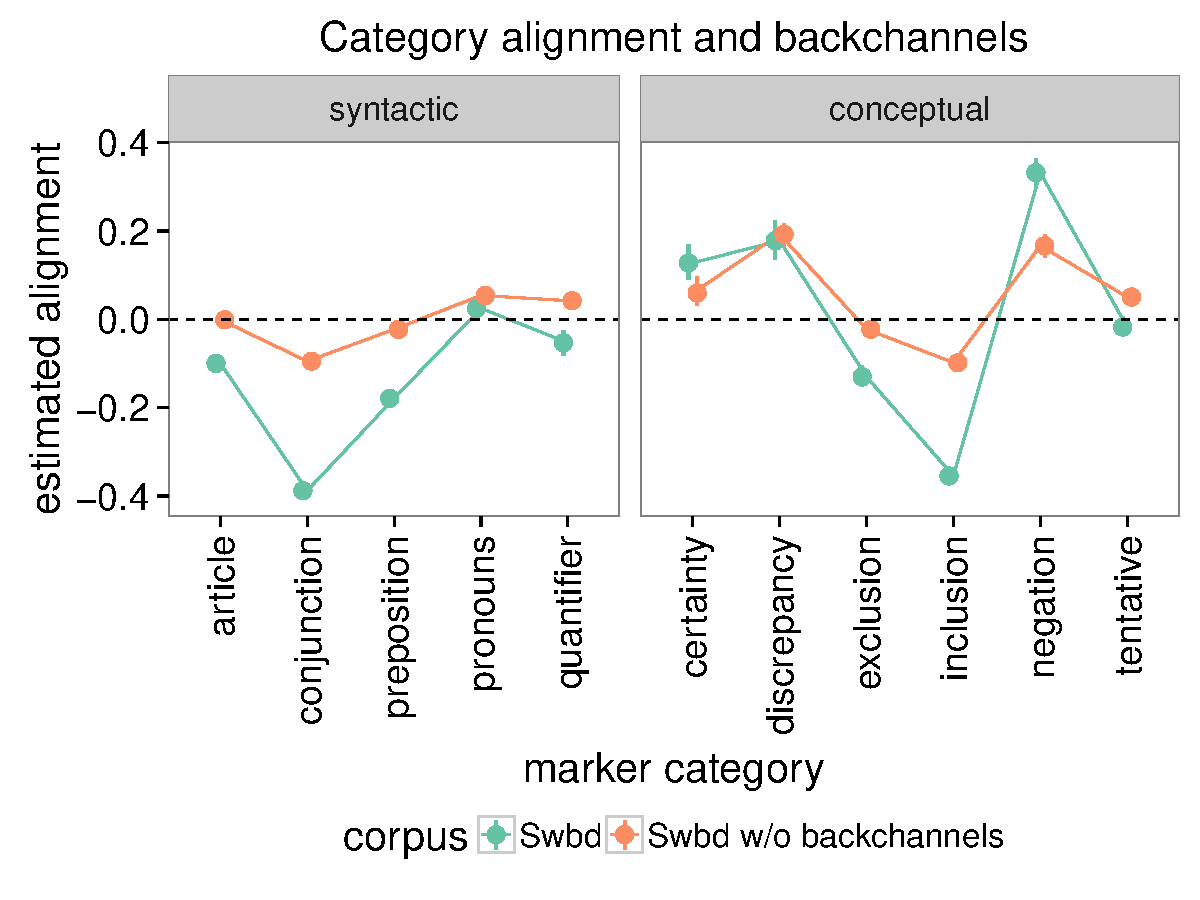
\includegraphics[width=\columnwidth]{results/swbds_line.pdf}\vspace{-10pt}
  \end{center}
  \caption{Comparing categorical alignment on the Switchboard dataset with and without backchannels. 95\% HPD intervals from WHAM shown.}\label{fig:swbds-res}
\end{figure}

Interestingly, the two categories that do show greater alignment when backchannels are included are certainty and negation. These categories are both important for backchannels; a negative backchannel is generally inappropriate in reply to a non-negative message, and similarly a confident backchannel would often be out of place in reply to an uncertain message. These influences of discourse acts on alignment are consistent with a discourse-strategic origin for alignment.

\section{Discussion}
Linguistic alignment is a prominent type of communicative accommodation, but its sources are unclear.  We presented WHAM, a length-robust extension of a probabilistic alignment model. Using this model, we find evidence that linguistic alignment is primarily lexical, and that it is strongly affected by at least some aspects of the discourse goal of a message.

This combination of a primarily-lexical origin for linguistic alignment and its variation by category and discourse acts suggest that alignment is primarily a higher-level discourse strategy rather than a low-level priming-based mechanism.  This set of results is consistent with both Accommodation Theory \cite{GilesCouplandCoupland1991} and the set of findings, reviewed above, that sociological factors affect the level of observed alignment.  The effect of  discourse acts on alignment further suggests that alignment is not a completely automatic process but rather one of many discourse strategies that speakers use to achieve their conversational goals.



%If category alignment is primarily lexical, what is the meaning of a category? The fact that category alignments can be estimated with small HPDs suggests that words in a category really do have similar alignment behavior, even though they largely don't affect each other.

%Backchannels are just one example of a discourse act that may interact with alignment; examining a wider range of discourse acts may reveal an important trade-off between conversational goals and alignment. The Switchboard discourse acts are classified in terms of their forward and backward communicative functions. Forward communicative functions in particular may interfere with alignment as the goals of advancing the conversation and of re-using structure from the preceding message conflict.


%\section*{Acknowledgments}
%
%The acknowledgments should go immediately before the references.  Do
%not number the acknowledgments section. Do not include this section
%when submitting your paper for review.

% include your own bib file like this:
%\bibliographystyle{acl}
%\bibliography{acl2016}
\newpage
\bibliography{disc_align.bib}
\bibliographystyle{acl2016}

\appendix

% \section{Supplemental Material}
% \label{sec:supplemental}

% (Temporary collection of material that I'm considering adding as supplemental material -- separate from the paper, doesn't count against 8-page limit. [references also don't count against limit])

% \begin{table}[h]
% \begin{center}
% \begin{tabular}{|c||c|c|c|c|}
% \hline
% %\bf & \bf \multicolumn{4}{c}{Reply} \\ \hline
% \bf Message & \{$\emptyset$\} & \{X\} & \{Y\} & \{X,Y\} \\ \hline
% \{$\emptyset$\} &  160 & 20 & 10 & 10\\
% \{X\} & 140 & 30 & 20 & 10 \\
% \{Y\} & 170 & 10 & 15 & 5 \\
% \hline
% \end{tabular}
% \end{center}
% \caption{\label{table:cnw-example2} Another case where (mean lexical) > categorical alignment.}
% \end{table}

% [Proof that LLA and Healey's measure of lexical similarity can depend on message/reply length.]

\end{document}
